\chapter{Introduction to lab equipment}\label{chap:intro}

The purpose of this lab is to introduce the computer programs and the
equipment you will be using in this course.  You will simulate the operation
of an open-loop motor scheme, illustrated in Figure~\ref{fig:openLoop1}\@.
\begin{figure}[htbp]
\centering
\begin{picture}(200,50)
\put(0,22){$u(t)$}
\put(20,25){\vector(1,0){30}}
\put(55,5){\framebox(105,40)
{\large\((\frac{d^2}{dt^2}+\frac{1}{\tau}\frac{d\theta}{dt})=k_Eu\)}}
\put(165,25){\vector(1,0){30}}
\put(196,22){\(\theta(t)\)}
\end{picture}
\caption{Open-loop motor schematic}\label{fig:openLoop1}
\end{figure}%
Hence, the differential equation governing the system is:
\begin{equation}\label{eq:motor}
\frac{d^{2}\theta}{dt^{2}}+\frac{1}{\tau}\frac{d\theta}{dt}=k_Eu.    
\end{equation}
We are interested in the angle, $\theta$\@, and the angular velocity,
$\omega=\frac{d\theta}{dt}$\@, of the motor shaft.  By the end of the lab,
you will have enough data to calculate the motor time constant, $\tau$\@, and
torque constant, $k_{E}$\@.

\section{Prelab}

It is assumed that the students of this course will have working knowledge of
personal computers. Before you go into the lab, you should read the
following:
\begin{itemize}
\item Appendix~\ref{chap:MATLAB}\@: \textsf{Matlab}\@;
\item Appendix~\ref{chap:hardware}\@: Lab equipment;
\item Appendix~\ref{chap:simulink}\@: \textsf{Simulink}\@;
\item Section~\ref{sec:motor} from the course text.
\end{itemize}
You will be expected to be able to look up material in the appendices during
the course of the various labs, so it is best that you be familiar with what
is in them.  If you are already familiar with any of the topics, you may skip
that section.

\section{Procedure}

The following steps should be followed to set up the simulink models to
properly communicate with the hardware.  You should perform the following
steps \emph{before} adding any blocks to your simulink model to avoid
manually configuring each block in your model.  Concerning any check boxes,
if it is not explicitly stated that you should check a box then it
\emph{must} be left unchecked.
\begin{enumerate}
\item Create the directory 
\begin{center}
\verb|C:\Documents and Settings\<Qlink ID>\My Documents\MATLAB|
\end{center} 
if it does not already exist.
\item Start \textsf{Matlab}.
\item Type \verb|simulink| at the prompt.
\item Click \verb|File|$\to$\verb|New|$\to$\verb|Model| to create a new empty
simulink model.
\item Build a \textsf{Simulink} model (the following steps will guide you
through this) as shown in Figure~\ref{fig:lab1}\@.
\begin{figure}[htbp]
\centering
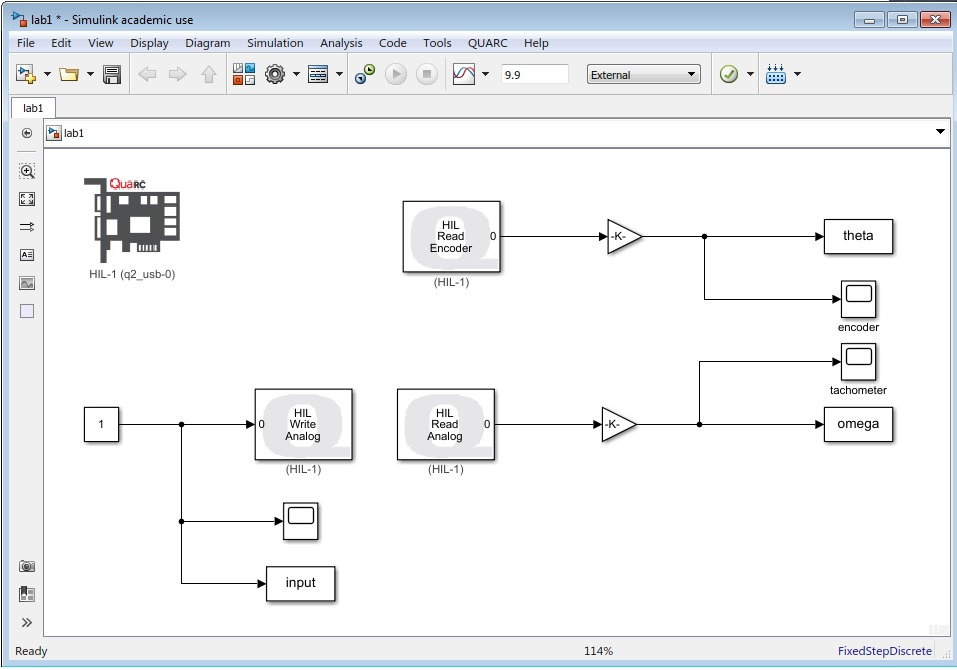
\includegraphics[width=0.9\textwidth]{pix/lab1.PNG} 
\caption{\textsf{Simulink} model for Lab~\ref{chap:intro}}\label{fig:lab1}
\end{figure}%
The model applies a constant voltage to the servomotor.  The encoder is
employed to acquire the angular position ($\theta$) and the tachometer is
used to acquire the angular velocity ($\omega$) as functions of time.
\item Make a new folder on the hard drive under the name or number of your
group and save your model under the name \verb|lab1_name_of_your_group.mdl|.
Save all files created (e.g., model file, plots) in each lab session in that
folder.  It might be a good idea to create a folder for each lab session as
well.

\item Drag the \verb|HIL Initialize| block from the library window into the
model.  You can find this block under:
\begin{center}
\verb|QuaRC Targets|$\to$\verb|Data Acquisition|$\to$\verb|Generic|$\to$\verb|Configuration|
\end{center}
\item Double click on the new \verb|HIL Initialize| block in your model to
configure the parameters.
\begin{enumerate}
\item Main Tab
\begin{itemize}
\item Board Type = \verb|q2_usb|
\end{itemize}
\item Encoder Inputs Tab
\begin{itemize}
\item Encoder Input Channel = \verb|[0]|
\item Encoder Quadrature = \verb|[4]|
\item Encoder Frequency in Hertz = \verb|[ ]|
\item Initial Encoder Counts = \verb|0|
\item Check box \verb|Set encoder input parameters at model start|
\item Check box \verb|Set initial encoder counts at model start|
\end{itemize}
\item Analog Outputs Tab
\begin{itemize}
\item Analog Output Channels = \verb|[0]|
\item Initial Analog Outputs = \verb|0|
\item Final Analog Outputs = \verb|0|
\item Analog Outputs on Watchdog Expiry = \verb|0|
\item Check box \verb|Set initial analog outputs when switching to this model|
\item Check box \verb|Set final analog outputs at model termination|
\item Check box \verb|Set final analog outputs when switching from this model|
\end{itemize}
\end{enumerate}

\item Click \verb|Apply| and then \verb|OK| to close the properties dialog box.

\item Once the \verb|HIL Initialize| block is set up properly, you can add
blocks to your simulink model to read and write analog signals to the
interface board.  The main blocks of interest are \verb|HIL Read Encoder|,
\verb|HIL Read Analog| and \verb|HIL Write Analog|, which replace the old
blocks \verb|Encoder Input|, \verb|Analog Input| and \verb|Analog Output|,
respectively.  Consult the instructions to see which blocks to use in each
lab. There are no \verb|calibration|, \verb|encoder|, or \verb|tachometer|
blocks.  These blocks are simply ``gain'' or ``scope'' blocks which have been
renamed.  It is always best to refer to the block pictures instead of the
block names.  These blocks can be found at
\begin{center}
\verb|QuaRC Targets|$\to$\verb|Data Acquisition|$\to$\verb|Generic|$\to$\verb|Immediate I/0|
\end{center}
\begin{center}
\verb|Simulink|$\to$\verb|Commonly used blocks|
\end{center}
When using the HIL \verb|Read Analog| block, make sure that the correct
channel is set (channel \verb|0|).
\begin{figure}[htbp]
\centering
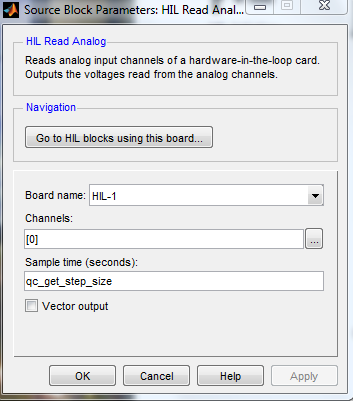
\includegraphics[width=0.5\textwidth]{pix/hil-read-analog-block.PNG}
\caption{HIL \texttt{Read Analog} block settings}\label{fig:hilrab}
\end{figure}
\begin{figure}[htbp]
\centering
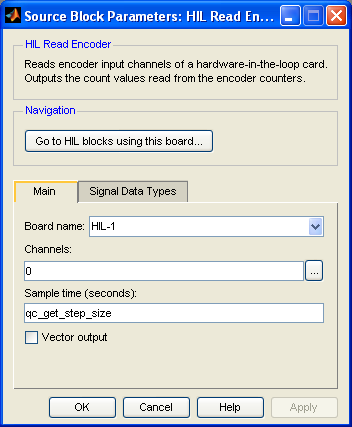
\includegraphics[width=0.5\textwidth]{pix/hil-read-encoder-block.PNG}
\caption{HIL \texttt{Read Encoder} block settings}\label{fig:hilreb}
\end{figure}
\begin{figure}
\centering
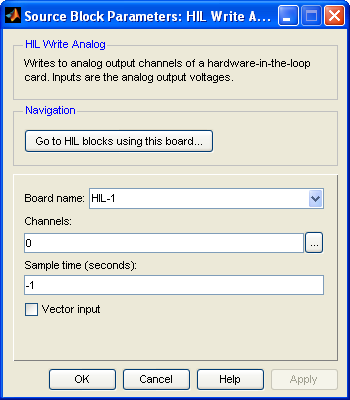
\includegraphics[width=0.5\textwidth]{pix/hil-write-analog-block.PNG}
\caption{HIL \texttt{Write Analog} block settings}\label{fig:hilwab}
\end{figure}
\item The input and output channel numbers in the \textsf{Simulink} blocks should
match the channels used on the terminal board. Refer to
Figures~\ref{fig:hilrab}\@,~\ref{fig:hilreb}\@, and~\ref{fig:hilwab} for the
correct channels.
\item \label{enum:parameters} The calibration factors need to be set so that
servomotor angular position and velocity are acquired in appropriate units.
Refer to Table~\ref{tab:conversionFactors} in Appendix~\ref{chap:hardware}
for calibration constants of the sensors.  These values are entered in the
appropriate \verb|Gain| blocks in the \textsf{Simulink} window.
\item The \verb|To Workspace| block can be found at
\verb|Simulink|$\to$\verb|Sinks|.  Drag this block into your workspace and
connect it to the variable you wish to save.  Double click on the block to
configure it.  Choose a good variable name and, in the \verb|save format|
drop down menu, select \verb|Structure with time|.
\item Click on \verb|Simulation|$\to$\verb|Configuration Parameters| from
your \textsf{Simulink} screen (or \verb|Ctrl+E|).  Make sure you are using
\verb|fixed-step| integration and choose \verb|ode 4| as your method.  Also
the software seems to forget all data older than 10 seconds during the
simulations, so it is often useful to set the stop time to 9.9 seconds.
\item Double click on the \verb|Encoder| and \verb|Tachometer| blocks to open
the plots.  More details on viewing real-time results can be found in
Appendix~\ref{chap:simulink}\@.
\item Select \verb|Set default options| from the \verb|QuaRC| drop down menu.
\item If your simulation involves hardware, then select the \verb|External|
mode option from the drop down menu in the toolbar. Otherwise choose normal.
\item Select \verb|Build| from the \verb|QuaRC| drop down menu.  Wait for
building to be completed before proceding to next step. Progress can be seen
in the Command Window.
\item Provided there are no compilation errors, select
\verb|Connect to Target| from the \verb|Simulation| menu.
\item Select \verb|Start Real Time Code| from the \verb|Simulation| menu.
\item Data will automatically be saved from the \verb|To Workspace| blocks.
\item Plot it with the command
\begin{center}
\verb|plot(varname.time,varname.signals.values)|
\end{center}
replacing ``\verb|varname|'' with the variable name you chose when
configuring the \verb|To Workspace| block.  Use the \verb|plot| command in
\textsf{Matlab} to plot data from the \verb|Encoder| and the
\verb|Tachometer|.  Details on plotting in \textsf{Matlab} are discussed in
Appendix~\ref{chap:MATLAB}\@.  Remember to give the plots appropriate title
and axis labels and print these plots. What is the steady state angular
velocity?  Are the results from these plots as you expected?
\item Now that you have obtained the steady-state value from the angular
velocity plot, you are ready to determine the actual value of the motor time
constant, $\tau$, and the torque constant, $k_{E}$\@.  Recall that solving
the differential equation~(\ref{eq:motor}) with zero initial condition yields
\begin{align}\notag
\omega(t)=&\;\dot\theta(t),\\\label{eq:motorSoln}
\omega(t)=&\;k_{E}\tau (1-e^{-t/\tau}),
\end{align}
and so the steady state value is just $k_{E}\tau$\@.
\item First, determine the steady state value and the constant $\tau$ from
the angular velocity plot.  You can find $\tau$ by using the steady state
value and finding the value of $\omega(t)$ when $t=\tau$\@.  Alternatively,
you can determine $\tau$ from the slope of the plot at $t=0$ (how?).
\item Next, determine $k_{E}$ using Equation~(\ref{eq:motorSoln}) and the
constants obtained in the last step.  You might need to zoom in to the
appropriate portion of the graph to see the result clearly.
\item Once you have confirmed with the TA that you have obtained the correct
value of the constants, print a copy of the plot that you zoomed in on.
\item Save all files in the folder you created.  Hand in all the plots you
printed during this lab session and along with it the work to show how you
have obtained the two constants.  Please make sure the names and student
numbers of all your group members are on the first page.
\end{enumerate}
The constants obtained in this lab will come in handy in the future, so make
sure you check with the TA that you have obtained the correct (or reasonably
close) value before you leave.

%%% Local Variables: 
%%% mode: latex
%%% TeX-master: "lab-manual"
%%% End: 
